\chapter{Desenvolvimento do experimento}

\iffalse introduction text \fi

\section{Preparação dos dados}

Os dois conjuntos de dados se encontravam em formato de texto, com os atributos separados por espaços e as instâncias separadas pelo caractere nova linha. A listagem \ref{lst:dev_data} mostra as primeiras cinco instâncias do \emph{Cr.Ger} no formato do arquivo original (a primeira coluna representa o número da linha, e não faz parte dos dados).

\vspace{0.5cm}
\begin{lstlisting}[caption=Formato original dos dados (\emph{Cr.Ger}), label=lst:dev_data]
A11 6 A34 A43 1169 A65 A75 4 A93 A101 4 A121 67 A143 A152 2 A173 1 A192 A201 1
A12 48 A32 A43 5951 A61 A73 2 A92 A101 2 A121 22 A143 A152 1 A173 1 A191 A201 2
A14 12 A34 A46 2096 A61 A74 2 A93 A101 3 A121 49 A143 A152 1 A172 2 A191 A201 1
A11 42 A32 A42 7882 A61 A74 2 A93 A103 4 A122 45 A143 A153 1 A173 2 A191 A201 1
A11 24 A33 A40 4870 A61 A73 3 A93 A101 4 A124 53 A143 A153 2 A173 2 A191 A201 2
\end{lstlisting}
\vspace{0.5cm}

A preparação dos dados para a importação no WEKA consistiu na adição de uma seção de cabeçalho e da formatação dos dados para valores separados por vírgula (seção \ref{sec:prop_arff}), e o resultado é mostrado nas listagens \ref{lst:dev_arff_ger} e \ref{lst:dev_arff_aust} (essas listagens mostram apenas as primeiras cinco instâncias na seção de dados).

\vspace{0.5cm}
\begin{lstlisting}[caption=Arquivo ARFF do \emph{Cr.Ger}, label=lst:dev_arff_ger]
@relation cr.ger

@attribute A1  {A11,A12,A13,A14}
@attribute A2  numeric
@attribute A3  {A30,A31,A32,A33,A34}
@attribute A4  {A40,A41,A42,A43,A44,A45,A46,A47,A48,A49,A410}
@attribute A5  numeric
@attribute A6  {A61,A62,A63,A64,A65}
@attribute A7  {A71,A72,A73,A74,A75}
@attribute A8  numeric
@attribute A9  {A91,A92,A93,A94,A95}
@attribute A10 {A101,A102,A103}
@attribute A11 numeric
@attribute A12 {A121,A122,A123,A124}
@attribute A13 numeric
@attribute A14 {A141,A142,A143}
@attribute A15 {A151,A152,A153}
@attribute A16 numeric
@attribute A17 {A171,A172,A173,A174}
@attribute A18 numeric
@attribute A19 {A191,A192}
@attribute A20 {A201,A202}
@attribute A21 {1,2}

@data
A11,6,A34,A43,1169,A65,A75,4,A93,A101,4,A121,67,A143,A152,2,A173,1,A192,A201,1
A12,48,A32,A43,5951,A61,A73,2,A92,A101,2,A121,22,A143,A152,1,A173,1,A191,A201,2
A14,12,A34,A46,2096,A61,A74,2,A93,A101,3,A121,49,A143,A152,1,A172,2,A191,A201,1
A11,42,A32,A42,7882,A61,A74,2,A93,A103,4,A122,45,A143,A153,1,A173,2,A191,A201,1
A11,24,A33,A40,4870,A61,A73,3,A93,A101,4,A124,53,A143,A153,2,A173,2,A191,A201,2
\end{lstlisting}
\vspace{0.5cm}

\vspace{0.5cm}
\begin{lstlisting}[caption=Arquivo ARFF do \emph{Cr.Aust}, label=lst:dev_arff_aust]
@relation cr.aust

@attribute A1  {0,1}
@attribute A2  numeric
@attribute A3  numeric
@attribute A4  {1,2,3}
@attribute A5  {1,2,3,4,5,6,7,8,9,10,11,12,13,14}
@attribute A6  {1,2,3,4,5,6,7,8,9}
@attribute A7  numeric
@attribute A8  {1,0}
@attribute A9  {1,0}
@attribute A10 numeric
@attribute A11 {1,0}
@attribute A12 {1,2,3}
@attribute A13 numeric
@attribute A14 numeric
@attribute A15 {0,1}

@data
1,22.08,11.46,2,4,4,1.585,0,0,0,1,2,100,1213,0
0,22.67,7,2,8,4,0.165,0,0,0,0,2,160,1,0
0,29.58,1.75,1,4,4,1.25,0,0,0,1,2,280,1,0
0,21.67,11.5,1,5,3,0,1,1,11,1,2,0,1,1
1,20.17,8.17,2,6,4,1.96,1,1,14,0,2,60,159,1
\end{lstlisting}
\vspace{0.5cm}

Com os arquivos no formato ARFF, os conjuntos de dados podem ser importados no WEKA. A figura \ref{fig:dev_weka_arff} mostra o conjunto de dados \emph{Cr.Ger} quando importado. Um conjunto de dados importado pode ser utilizado para qualquer algoritmo que suporte os tipos de atributos contidos nele.

\vspace{0.5cm}
\begin{figure}[h!]
    \centering
    \caption{Conjunto de dados \emph{Cr.Ger importado no WEKA}}
    \label{fig:dev_weka_arff}
    \vspace{0.5cm}
    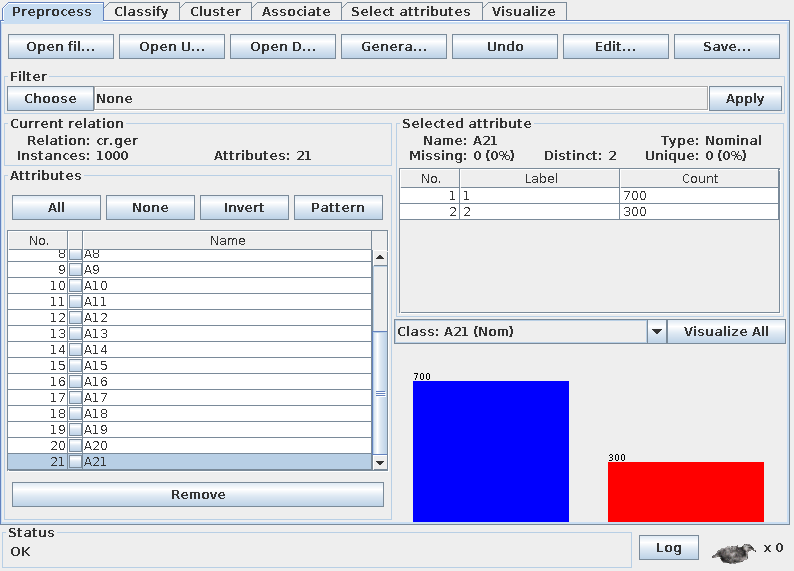
\includegraphics[width=0.75\textwidth]{img/cr_ger.png}
    \vspace{0.5cm}
\end{figure}
\vspace{0.5cm}

\section{Utilizando o WEKA}

\subsection{Interfaces}

O WEKA apresenta duas interfaces principais: linha de comando e gráfica (Interface Gráfica, GUI\nomenclature{GUI}{Graphical User Interface}). A interface gráfica é mais apropriada para exploração e experimentação, e para a apresentação dos dados, algoritmos e resultados. Porém, para usos mais avançados e experimentos mais complexos, a linha de comando é mais apropriada. Além da possibilidade muito maior de automação de tarefas e exposição de opções avançadas que não estão disponíveis na interface gráfica, essa interface consume menos recursos.

Nesse trabalho foi utilizada a interface por linha de comando, já que a repetição dos testes para cada algoritmo é muito mais fácil do que se utiliza-se a interface gráfica. Os exemplos de execução são apresentados conforme devem ser digitados em uma interface de linha de comando, em um emulador de terminal, utilizando um \emph{shell} como \emph{sh} ou \emph{bash}.

\subsection{Out of Memory}

Todas as aplicações java possuem um limite máximo de memória que pode ser alocado por cada processo da máquina virtual java (Java Virtual Machine, JVM\nomenclature{JVM}{Java Virtual Machine}). Caso não seja especificado, o valor padrão de 64\emph{mb} é utilizado. Para a maioria das aplicações, esse valor é insuficiente. É possível alterar esse valor através da opção \emph{-Xmx} para o executável, passando como parâmetro o novo valor para o limite. Para utilizar 4\emph{gb} como limite, por exemplo, pode-se utilizar as seguintes notações, onde \emph{k} e \emph{m} significam \emph{kilo} e \emph{mega}, respectivamente:

\vspace{0.5cm}
\begin{lstlisting}[caption=Opções para aumentar o limite de meória da JVM, label=lst:dev_java_xmx]
java -Xmx4294967296
java -Xmx4194304k
java -Xmx4096m
\end{lstlisting}
\vspace{0.25cm}
\centerline{Fonte: \cite{Oracle1995}}
\vspace{0.5cm}

\subsection{Filtros}

No WEKA, um filtro é um objeto que recebe um conjunto de dados como entrada e produz um conjunto de dados modificado. Esse é um processo comum da Mineração de Dados, chamado de pré-processamento dos dados: adicionar, remover ou alterar atributos, etc.

Um filtro comum, que é utilizado nesse trabalho, é o de criação de partições para o \emph{cross-validation}. Para esse filtro, são passados três argumentos. O argumento \emph{c} indica qual dos atributos é o atributo correspondente à classe, e é representado por um índice, iniciado em 1, conforme a declaração na seção de atributos do arquivo de dados (caso o padrão do WEKA seja usado, ou seja, o atributo de classe seja o último da listagem, pode ser utilizado o valor ``\emph{last}'' como argumento). O argumento \emph{N} indica o número de partições, e o argumento \emph{F} indica a partição selecionada.

Além desses, o argumento \emph{V} pode ser utilizado para gerar o conjunto inverso de seleções, útil para dividir o conjunto em duas partes complementares. Dessa forma, para gerar um conjunto de dados para testes e outro para treinamento, podem ser usados os seguintes comandos\footnote{Nesses exemplos, é usado o redirecionamento de entrada e saída presentes na maioria dos \emph{shells} UNIX. O caractere ``<'' seguido de um nome de arquivo indica que aquele arquivo será usado como entrada para o comando. De maneira semelhante, o caractere ``>'' seguido de um nome de arquivo indica que ele será usado como saída. O WEKA também permite que sejam utilizadas as opções \emph{i} e \emph{o}, respectivamente, para obter os mesmos resultados. No primeiro exemplo, a forma equivalente seria ``\emph{-i dataset.arff -o dataset\_test.arff}''.}:

\begin{lstlisting}[caption=Filtro para geração de partições para \emph{cross-validation}, label=lst:dev_filter]
java weka.filters.supervised.instance.StratifiedRemoveFolds -c last -N 4 -F 1 \
    < dataset.arff > dataset_test.arff
java weka.filters.supervised.instance.StratifiedRemoveFolds -c last -N 4 -F 1 -V \
    < dataset.arff > dataset_train.arff
\end{lstlisting}

\subsection{Execução de um teste}

A execução de um algoritmo é feita através da classe que implementa o algoritmo no WEKA. Diversas opções podem ser passadas na linha de comando para mudar os parâmetros do algoritmo. Existem algumas opções adicionais para especificar dados adicionais, como os arquivos de dados para treinamento e testes. Além das opções gerais, cada algoritmo pode aceitar diferentes tipo de opções específicas. Como exemplo, para gerar a saída da listagem \ref{lst:prop_weka_out}, foi utilizado o comando da listagem \ref{lst:dev_exec_classifier}.

\vspace{0.5cm}
\begin{lstlisting}[caption=Execução de um classificador, label=lst:dev_exec_classifier]
java weka.classifiers.neural.lvq.Lvq1 -t data/weather.numeric.arff -i
\end{lstlisting}
\vspace{0.5cm}

Como é possível ver, a linha de comando é reproduzida no atributo ``\emph{Scheme}'' na saída. Esse atributo pode ser consultado para executar exatamente o mesmo teste novamente, tornando a reprodução do experimento muito mais fácil. As diversas opções do atributo que não estão presentes na linha de comando são os parâmetros do algoritmo. Como não foram especificados na linha de comando, foram assumidos os valores padrão, que são mostrados na saída. As duas opções que não estão presentes na saída são a opção ``\emph{i}'', que mostra uma saída mais complete e a opção ``\emph{t}'', que indica o arquivo que será utilizado como entrada.

Para executar os algoritmos do pacote de algoritmos imunológicos, é necessário informar à maquina virtual a localização do arquivo que contém o código executável. Esse código é disponibilizado em um arquivo \emph{jar}, um tipo de arquivo específico da linguagem java que é semelhante a um arquivo compactado utilizando os programas \emph{tar} ou \emph{zip}.

Para indicar que esse arquivo deve ser utilizado, é utilizada a opção \emph{classpath} da máquina virtual. Essa opção pode ser utilizada tanto para indicar um diretório quanto um arquivo \emph{jar}. Alternativamente, o arquivo \emph{jar} pode ser descompactado e o diretório gerado utilizado. Essa opção pode ser passada na linha de comando ou como uma variável de ambiente. Para executar o algoritmo AIRS, por exemplo, é utilizado qualquer um dos comandos da listagem \ref{lst:dev_weka_airs}. A sintaxe da opção \emph{classpath} é semelhante ao \emph{path} da maioria dos sistemas operacionais, ou seja, uma lista dos caminhos e arquivos separados pelo caractere ``:'' (dois-pontos).

\vspace{0.5cm}
\begin{lstlisting}[caption=Execução de um algoritmo do pacote de algoritmos imunológicos, label=lst:dev_weka_airs]
# Opção na linha de comando.
java -classpath wekaclassalgos.jar weka.classifiers.immune.airs.AIRS1 # parâmetros
# Variável de ambiente.
CLASSPATH=wekaclassalgos.jar
java weka.classifiers.immune.airs.AIRS1 # parâmetros
\end{lstlisting}
\vspace{0.5cm}

Combinando os conceitos apresentados nessa seção, a execução de um teste para um algoritmo imunológico utilizando um dos conjuntos de dados é feita de acordo com a listagem \ref{lst:dev_weka_single}. Aqui, é usado a opção ``\emph{t}'' para especificar o conjunto de dados \emph{Cr.Ger}. Todas as outras opções são parâmetros do filtro (os valores utilizados são os valores padrão para esse algoritmo).

\vspace{0.5cm}
\begin{lstlisting}[caption=Execução de um algoritmo do pacote de algoritmos imunológicos utilizando um dos conjuntos de dados, label=lst:dev_weka_single]
# Variável de ambiente.
CLASSPATH=wekaclassalgos.jar
java weka.classifiers.immune.airs.AIRS1 \
    -S 1 -F 0.2 -C 10.0 -H 2.0 -M 0.1 -R 150.0 -V 0.9 -A -1 -B 1 -E 1 -K 3 \
    -t german.arff
\end{lstlisting}
\vspace{0.5cm}
